\documentclass{ujarticle}
\usepackage{abstract}
\usepackage[dvipdfmx]{graphicx}
\usepackage{float} % これを追加

% ヘッダーを出力しない
\pagestyle{empty}

% ヘッダーを出力する場合は以下を設定
%\pagestyle{myheading}
%\kind{最終}% 中間 or 最終
%\year{4}% 年度
%\num{10}% No.

\title{剣道における熟練者の視線解析に基づくVRトレーニングシステムの構築} %タイトル
\author{吉田 隼人}% 報告者
\adviser{尾山 匡浩}% 指導教員

\begin{document}%

\maketitle % タイトルページの出力

\section{はじめに}%
%「スポーツビジョン」という言葉に象徴されるように、視覚機能はスポーツの上達における
%極めて重要な要素の一つである。視覚情報の適切な処理と判断を向上させるトレーニングは、
%球技のみならず武道を含む幅広い競技において必要不可欠とされている。

近年ではICT技術のスポーツへの導入が加速している。しかし、これらの多くは
球技などに焦点が当てられており、
武道におけるICT活用事例は未だ少ない。

剣道におけるICT活用研究として、
鳥越らによる慣性センサを用いた素振り解析\cite{torigoe}や、
Jeongらによるグリップ圧計測\cite{jeong}などが報告されているが、
これらは主に身体動作や力学的な定量化に留まっており、
競技の核心である「視覚」や「認知」には焦点が当てられていない。

一方で、視線に関する研究として秋山らによる熟練者の
メカニズム解明\cite{akiyama}が挙げられるものの、
その知見は現象の解析に終始しており、
実際のトレーニングに応用するための
具体的な「フィードバック手法」は未だ確立されていない。

本研究の最終目的は、XR技術とAIによる視線推定技術を統合し、熟練者の
視線情報を初学者が追体験できる新しい視線トレーニングシステムを構築することである。
その実現に向けた第一段階として、本研究では以下の二点を達成することを目的とする。
\begin{enumerate}
    \item 熟練者の視線を可視化するYOLOベースの解析手法の確立
    \item VR空間での視線追体験システムのベースの構築と、その動作検証
\end{enumerate}
%熟練者の視線を可視化するYOLOベースの解析手法の確立、および
%VR空間での視線追体験システムのベースの構築と、その動作検証
%という二点を達成することを目的とする。
%\begin{enumerate}
%    \item 熟練者の視線を可視化するYOLOベースの解析手法の確立
%    \item VR空間での視線追体験システムのベースの構築と、その動作検証
%\end{enumerate}

\section{提案システム}%
本研究で構築する剣道トレーニングシステムの構成を図\ref{nagare}に示す。
以下に各フェーズの詳細を述べる。
    \begin{figure}[h]
        \centering
        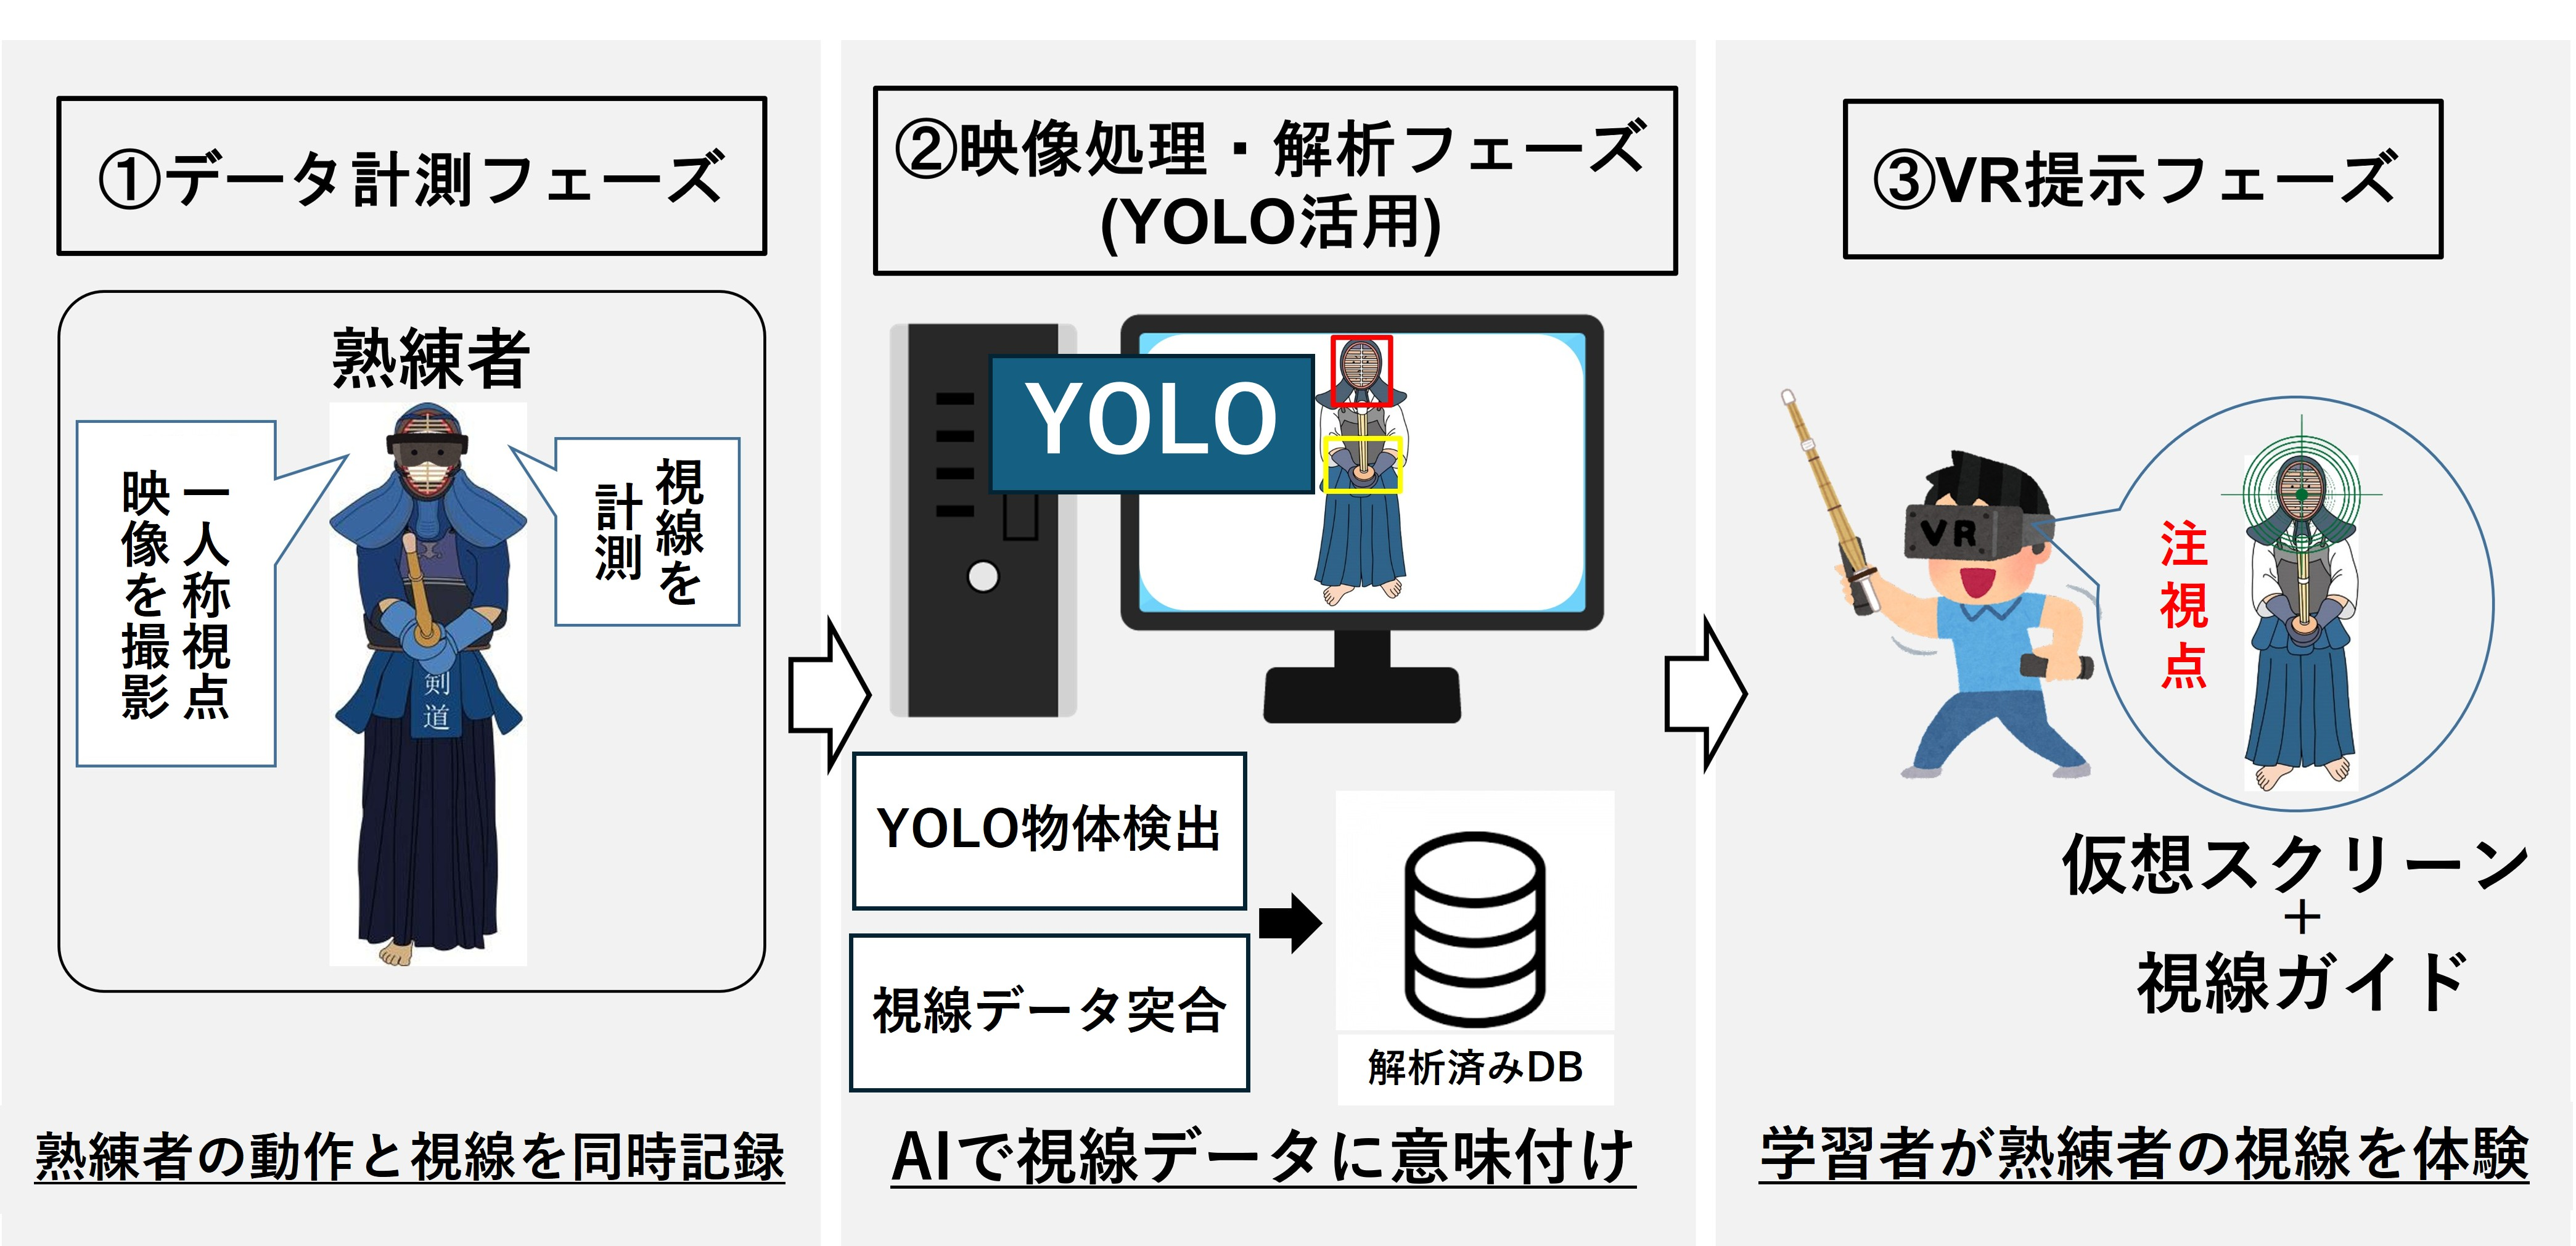
\includegraphics[width=1\columnwidth]{image_1_1.jpg}
        \caption{システム構成図}
        \label{nagare}
    \end{figure}

フェーズ1では、熟練者の視線技術を記録するためのデータ計測を行う。
実験協力者はウェアラブル型アイトラッカー「Pupil Invisible」を装着した状態で
実際の稽古を実施し、一人称視点映像と視線座標データの2種類を取得する。

次に、フェーズ2では映像処理・解析を行う。
視線の分布を可視化するために、YOLO11により人物検出を行い、
OpenCVとNumPyを用いてヒートマップを作成する。
具体的な処理手順を図\ref{fig:yolo_flow}に示す。

    \begin{figure}[h]
        \centering
        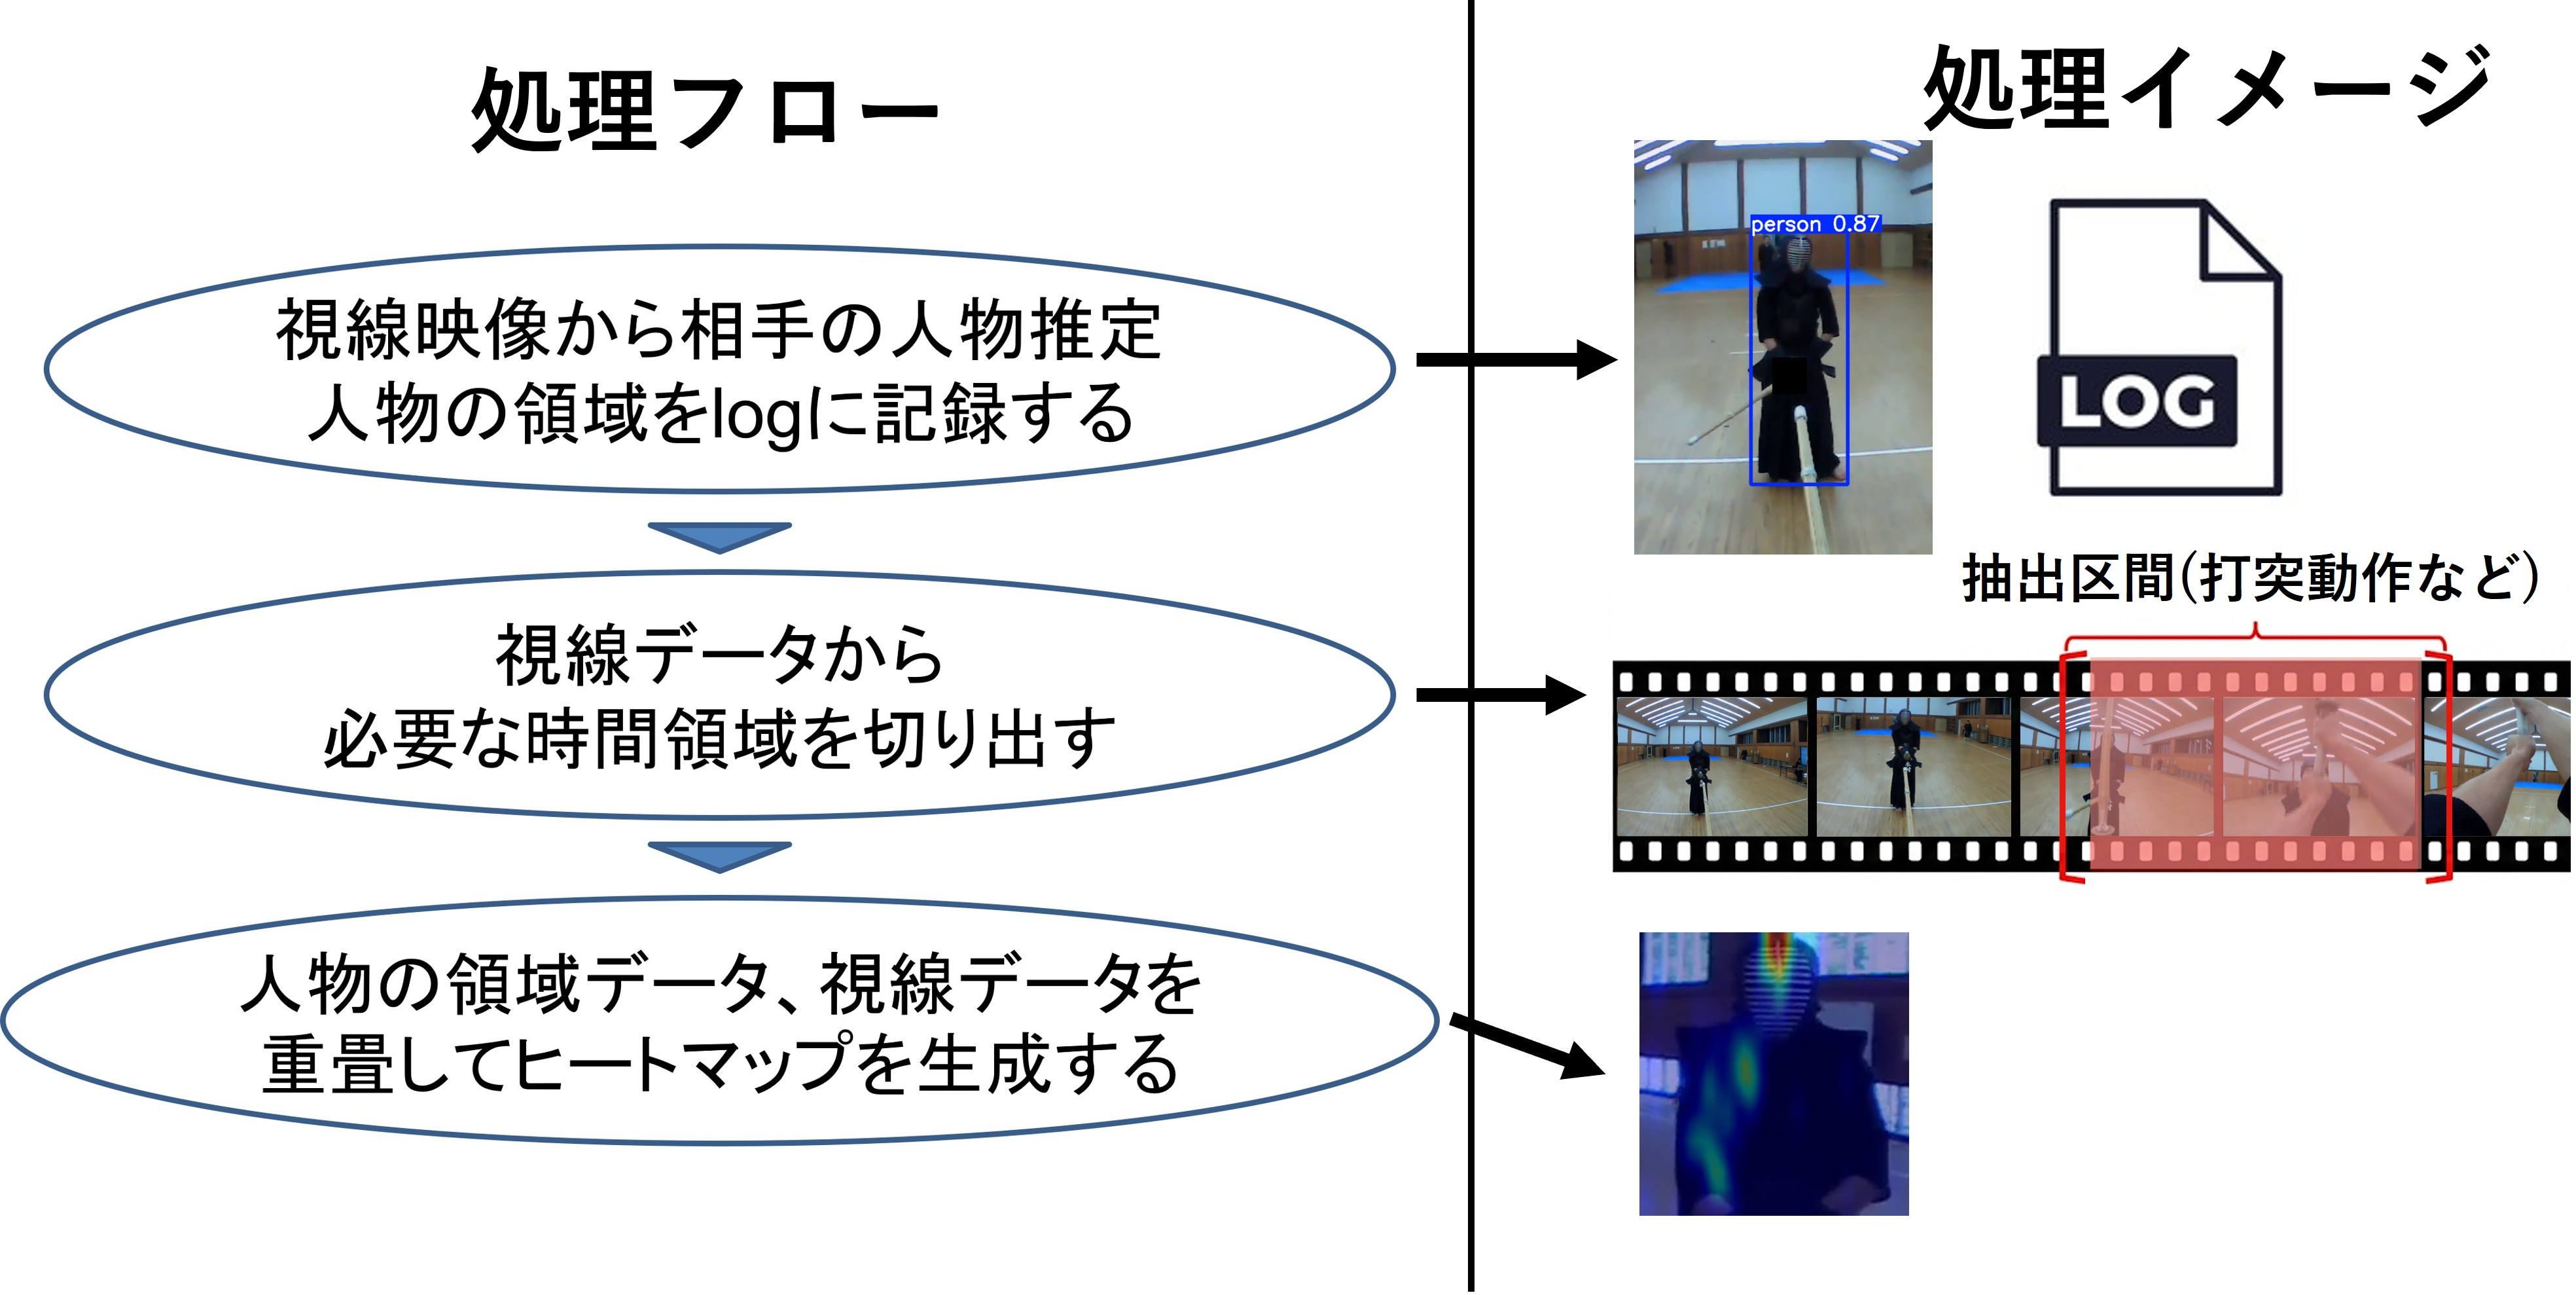
\includegraphics[width=1\columnwidth]{image_12_1.jpg} % スライド16枚目のフローチャート
        \caption{YOLO11を用いたヒートマップ生成フロー}
        \label{fig:yolo_flow}
    \end{figure}

    本手法を適用した結果を図\ref{18}に示す。
    激しい動きの中でも対戦相手の領域を正確に追従し、
    注視が集まっている様子を可視化することに成功した。

    \begin{figure}[h]
        \centering
        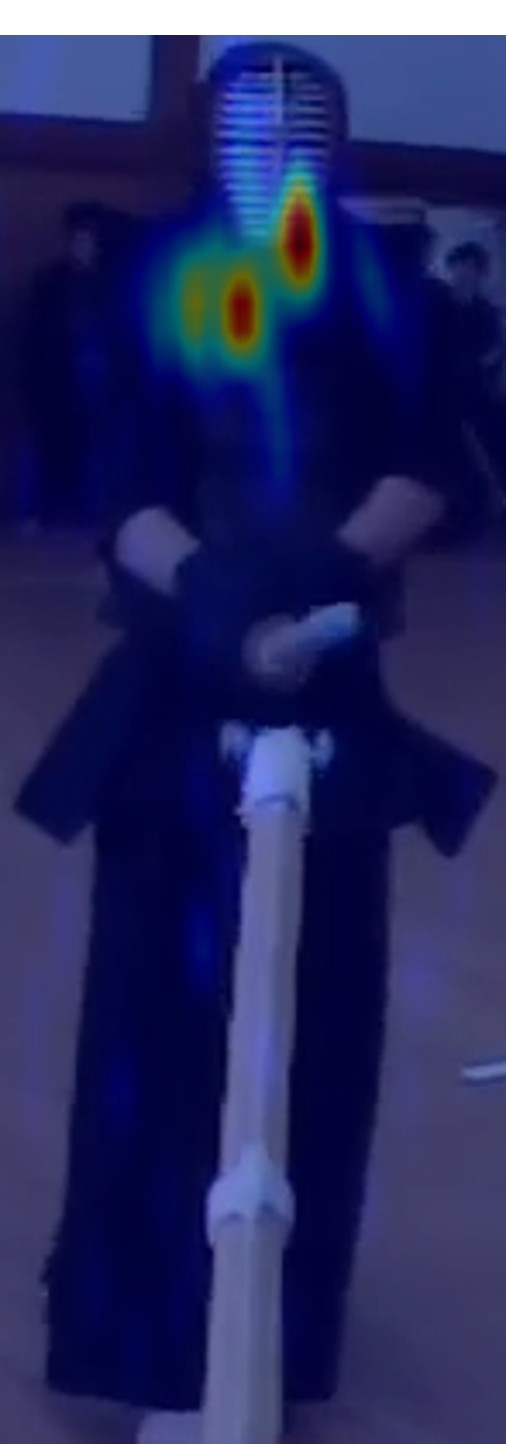
\includegraphics[width=0.25\columnwidth]{image_18_1.jpg} % スライド16枚目の検出画像
        \caption{提案手法(YOLO11)による生成結果}
        \label{18}
    \end{figure}

最後に、フェーズ3ではVR空間への実装と提示を行う。
前フェーズで記録した熟練者の視線データを重畳した映像を、
Unityを用いて構築したVR空間内に実装する。

%\subsection{フェーズ1：データ計測}
%熟練者の視線技術をデータとして保存する。被験者はウェアラブル型アイトラッカー
%「Pupil Invisible」を装着し、実際の稽古を行い、
%一人称視点映像と視線座標データの2種類が記録される。

%\subsection{フェーズ2：映像処理・解析}
%視線の分布をわかりやすく可視化するために、
%OpenCVとNumPyを用いてヒートマップを作成した。

%\subsection{フェーズ3：VR空間への実装と提示}
%前節で記録した熟練者の視線データが重畳された映像を、Unityを用いて構築したVR空間内へ実装した。

%\section{結果および考察}
%\subsection{データ計測実験}
%\subsubsection{実験条件}
%\begin{itemize}
%    \item \textbf{実験協力者}：男性（19歳、剣道二段）
%    \item \textbf{使用機材}：Pupil Invisible（視線計測）、
%    \item \textbf{動作課題}：対人形式での「面打ち」動作を含む基本稽古
%\end{itemize}
%実験協力者は19歳、剣道二段を保有する男性である。視線計測の使用機器として
%Pupil Invisibleを使用した。動作課題として対面形式での面うちを行った。
%取得したデータは視線計測デバイスからPupil Cloudにアップロードされた後、
%PCへとダウンロードされた。

%\subsection{ヒートマップ生成手法の比較と確立}
%\subsubsection{Pupil Cloudによるヒートマップ生成の検証}
%    Pupil Invisibleに標準付属するクラウド解析サービス
%    「Pupil Cloud」の有効性を示すため、
%    静止物体を対象とした予備実験を行った。
%    Pupil Cloudにおいてヒートマップを生成するためには、
%    スキャンビデオ、参照画像、視線計測データの3つのデータセットが必要である。
%    予備実験では、研究室内の「電気ポット」および「電子レンジ」を
%    対象に計測を行った。
%    結果として、Pupil Cloudのアルゴリズムが背景の特徴点を正しく追跡し、
%    参照画像と動画フレームのマッチングに成功した。
%
%\subsubsection{剣道映像への適用と課題}
%同様の手法を剣道の実技データに適用した。しかし、正常なヒートマップを生成することができなかった。
%生成失敗の主な原因は、剣道特有の動作にあると考えられる。
%剣道の競技中には急激な移動が伴い、一人称視点映像の背景が激しく変化する。そのため、
%特徴点マッチングに失敗し、生成エラーとなった。
%この結果より、
%標準機能であるPupil Cloudは本研究のような動的なスポーツシーンには不向きであると判断した。

%\subsection{YOLO11を用いた提案手法の実装}
%物体検出アルゴリズム「YOLO11」を用いた独自のヒートマップ
%生成パイプラインを構築した。
%具体的な処理手順を図\ref{fig:yolo_flow}に示す。

%    \begin{figure}[h]
%        \centering
%        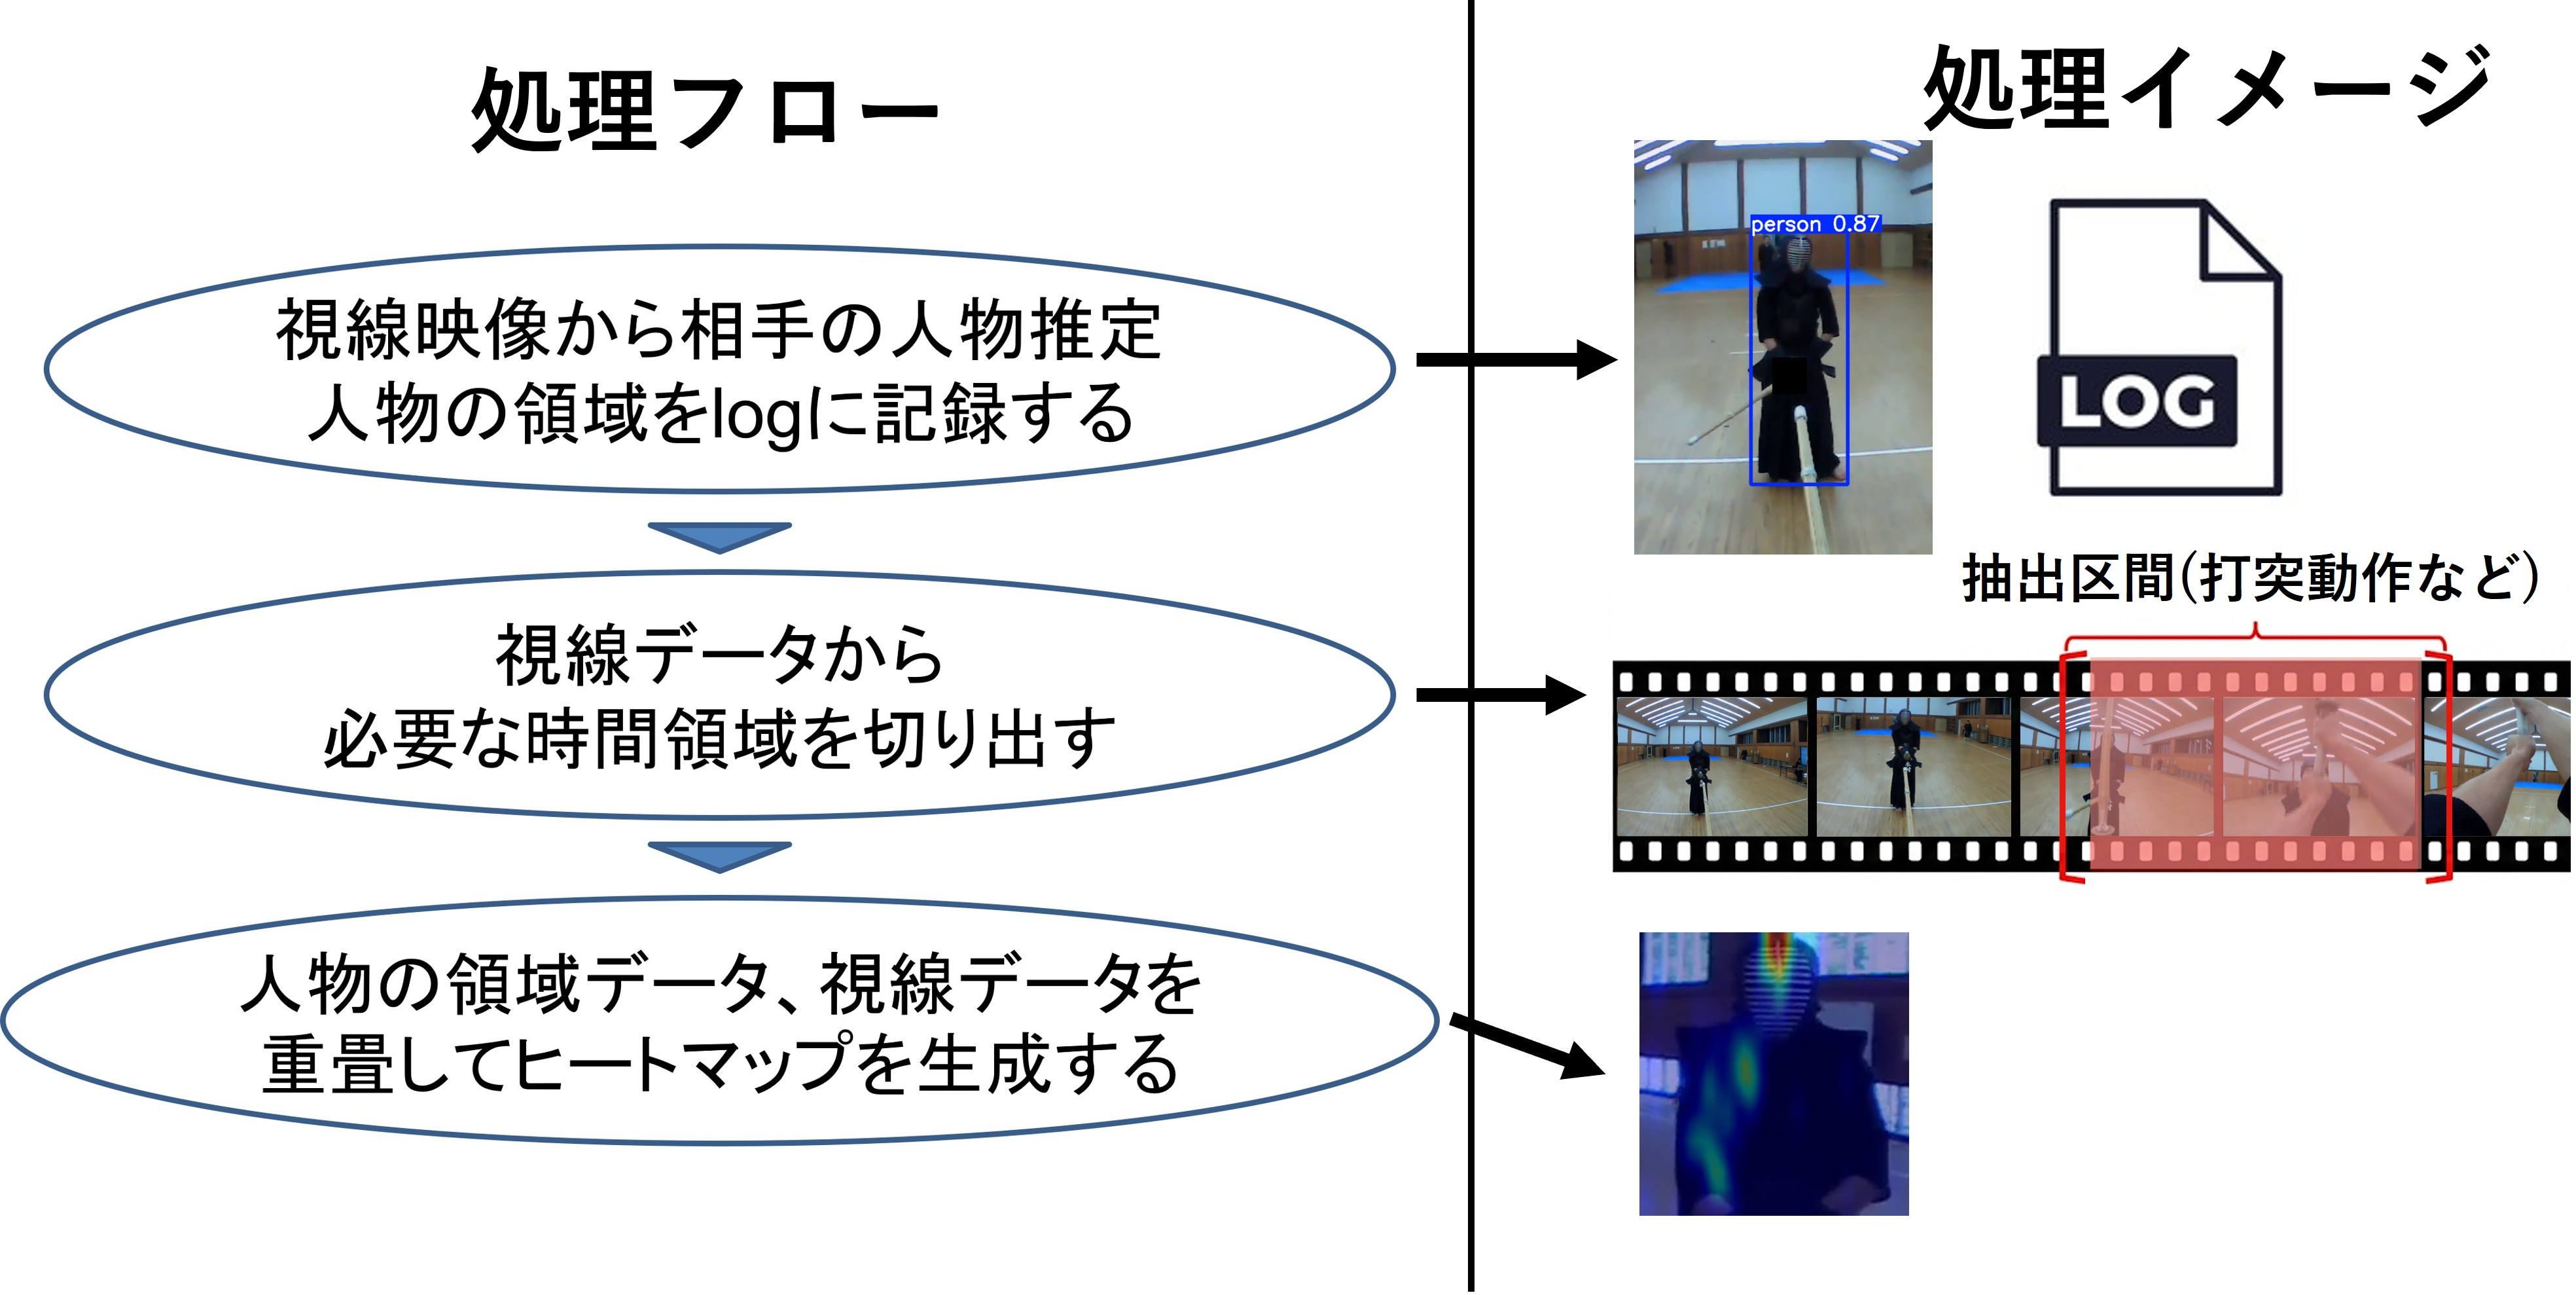
\includegraphics[width=1\columnwidth]{image_12_1.jpg} % スライド16枚目のフローチャート
%        \caption{YOLO11を用いたヒートマップ生成フロー}
%        \label{fig:yolo_flow}
%    \end{figure}

%    \subsubsection{1. 人物領域の特定とフィルタリング}
%    一人称視点映像の各フレームに対しYOLO11を適用し、人物クラスを検出する。
%    YOLO11による画像解析によって対戦相手として認識させたものから、
%    バウンディングボックス座標
%    （左上の$x, y$座標および幅$w$、高さ$h$）をログに記録する。
%
%    \subsubsection{3. 時間領域の同期と切り出し}
%    視線データと映像データのタイムスタンプを同期させ、
%    打突動作が行われている必要な時間領域のみを切り出す。
%
%    \subsubsection{4. 座標統合と描画}
%    記録した人物の領域データと視線座標データをフレームごとに統合する。
%    抽出した人物画像のバウンディングボックス内における視線位置の密度を計算し、
%    ヒートマップとして映像に重畳描画する。

%    本手法を適用した結果を図\ref{18}に示す。
%    激しい動きの中でも対戦相手の領域を正確に追従し、
%    注視が集まっている様子を可視化することに成功した。

%    \begin{figure}[h]
%        \centering
%        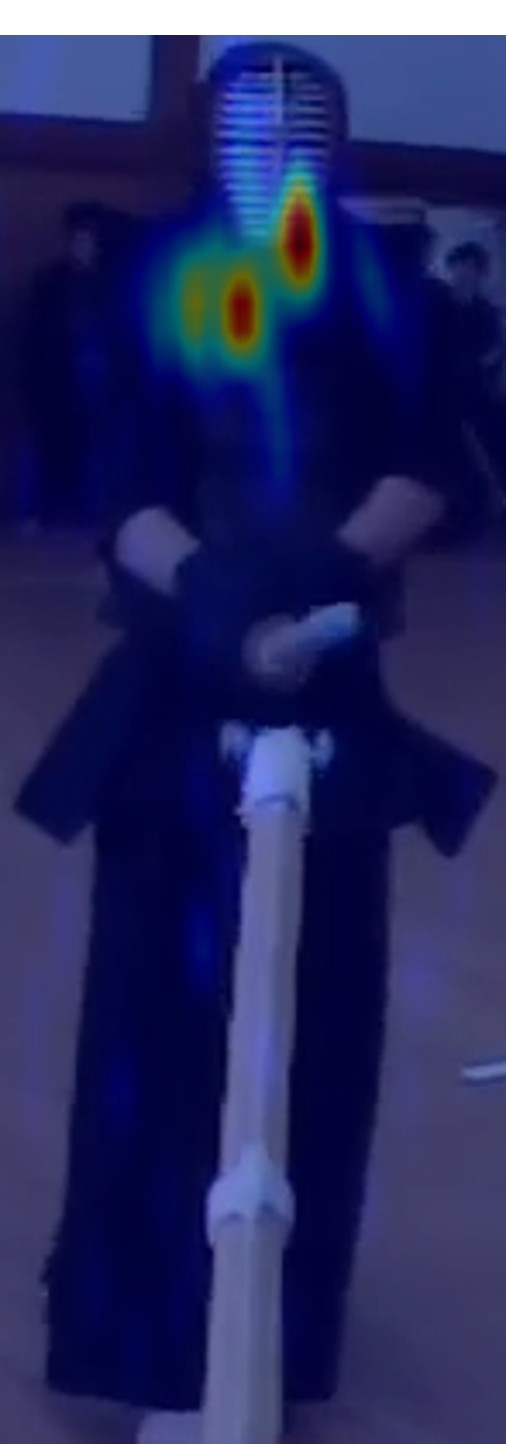
\includegraphics[width=0.2\columnwidth]{image_18_1.jpg} % スライド16枚目の検出画像
%        \caption{提案手法(YOLO11)による生成結果}
%        \label{18}
%    \end{figure}

\section{評価実験}
\subsection{条件}
    本提案手法を用いて、複数の実験協力者による面打ち動作時の視線データを可視化し、
    その傾向を分析した。
    実験に参加した実験協力者四名の属性を表\ref{tab:subjects_attribute}に
    示す。
    なお、実験では、実験協力者は面を被らずにPupil Invisibleを装着し、
    一回の計測につき面打ち動作を二回実施した。

    \begin{table}[htbp]
        \centering
        \caption{実験協力者の属性と特徴}
        \label{tab:subjects_attribute}
        \begin{tabular}{l|ccccc}
            \Hline
            & 性別 & 段位 & 経験年数 & 身長(cm) & 得意技 \\
            \hline
            A & 男 & 6段 & 25 & 169 & 面 \\
            B & 男 & 3段 & 13 & 180 & 小手 \\
            C & 男 & 3段 & 6 & 165 & 面 \\
            D & 男 & 2段 & 5 & 181 & 面 \\
            \hline
        \end{tabular}
    \end{table}

    \subsection{結果}

    本実験で計測したデータから提案手法により生成した各実験協力者の
    視線ヒートマップを図\ref{fig:compare_four_experts}に示す。

    \begin{figure}[htbp]
    \centering
    % 1人目
    \begin{minipage}{0.22\columnwidth}
        \centering
        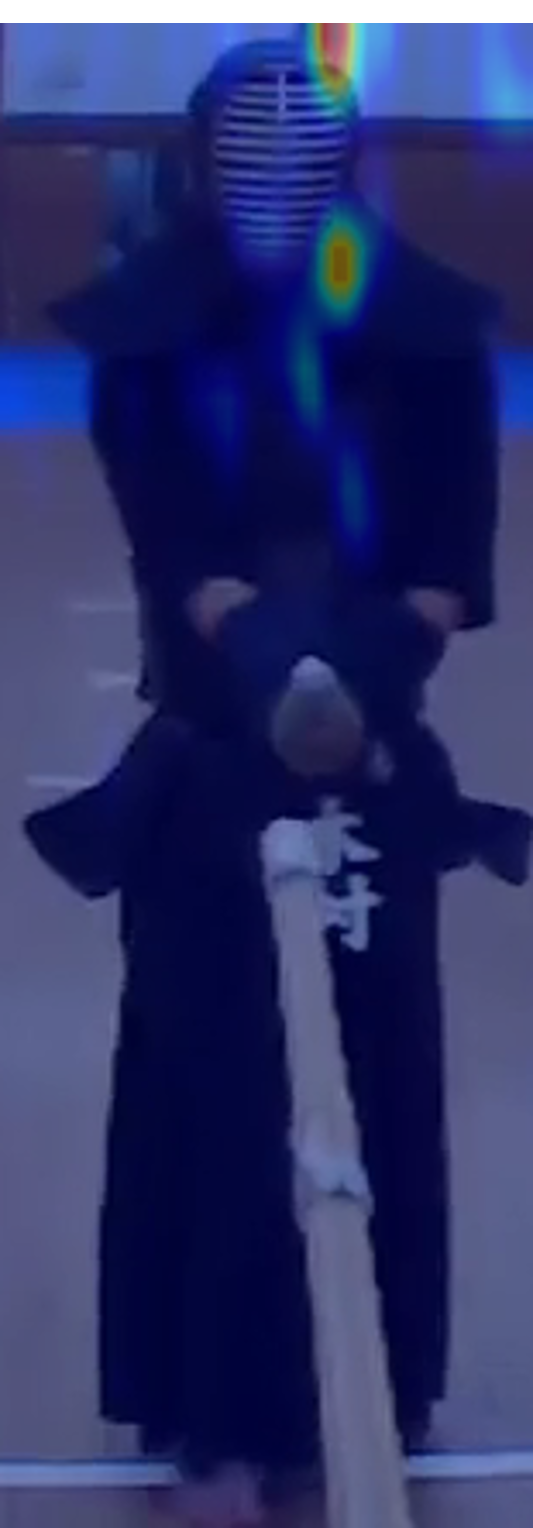
\includegraphics[width=\linewidth]{kcct-kc-01_head1__heatmap2_1.png}
        \par\vspace{2mm} % 画像との間隔を調整
        (A)
    \end{minipage}
    \hfill
    % 2人目
    \begin{minipage}{0.22\columnwidth}
        \centering
        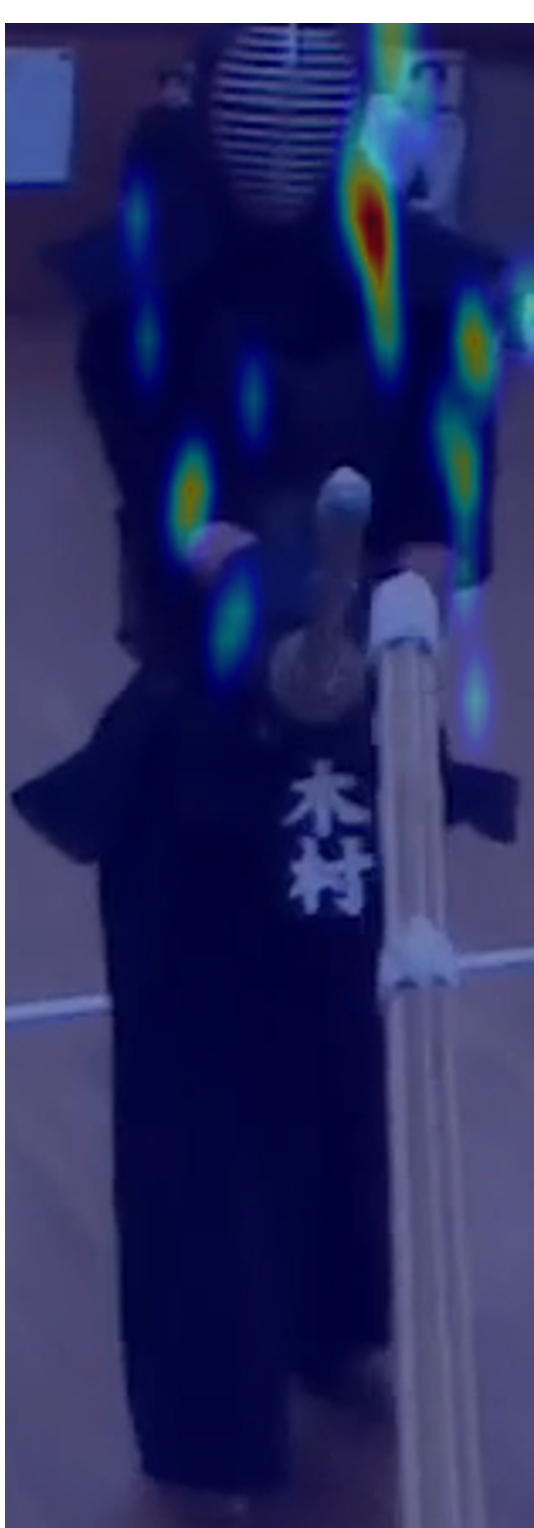
\includegraphics[width=\linewidth]{kcct-kc-02_head1__heatmap2_1.png}
        \par\vspace{2mm}
        (B)
    \end{minipage}
    \hfill
    % 3人目
    \begin{minipage}{0.23\columnwidth}
        \centering
        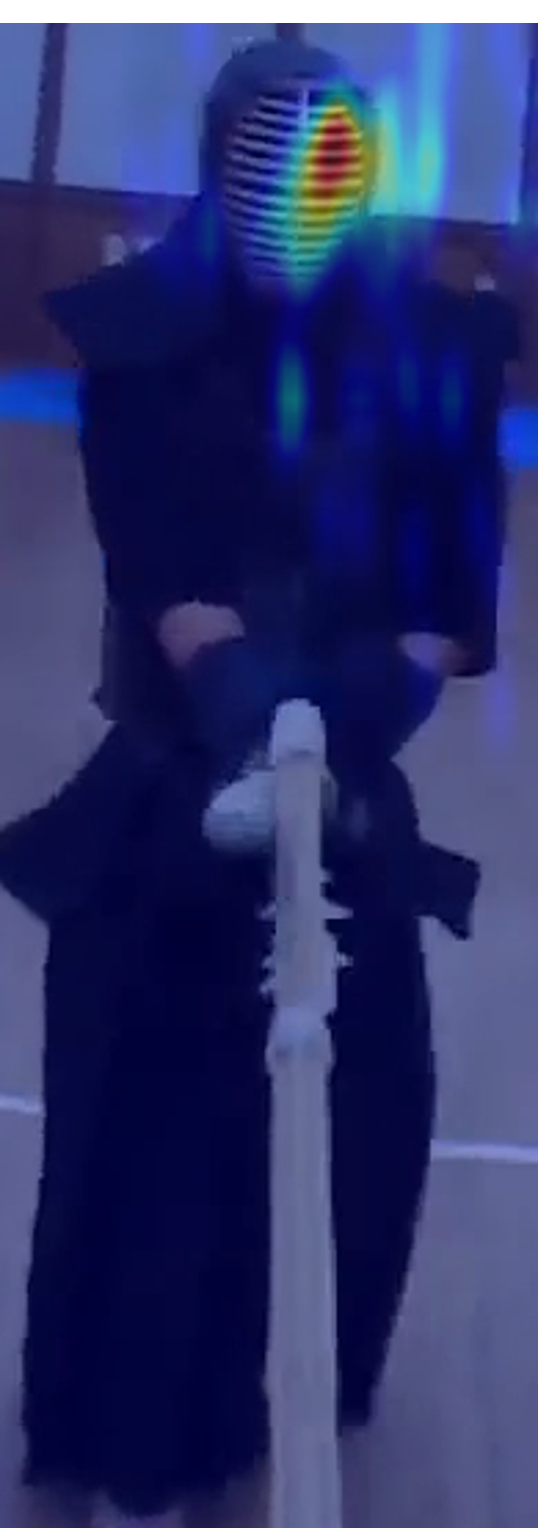
\includegraphics[width=\linewidth]{kcct-kc-04_head1__heatmap2_1.png}
        \par\vspace{2mm}
        (C)
    \end{minipage}
    \hfill
    % 4人目
    \begin{minipage}{0.23\columnwidth}
        \centering
        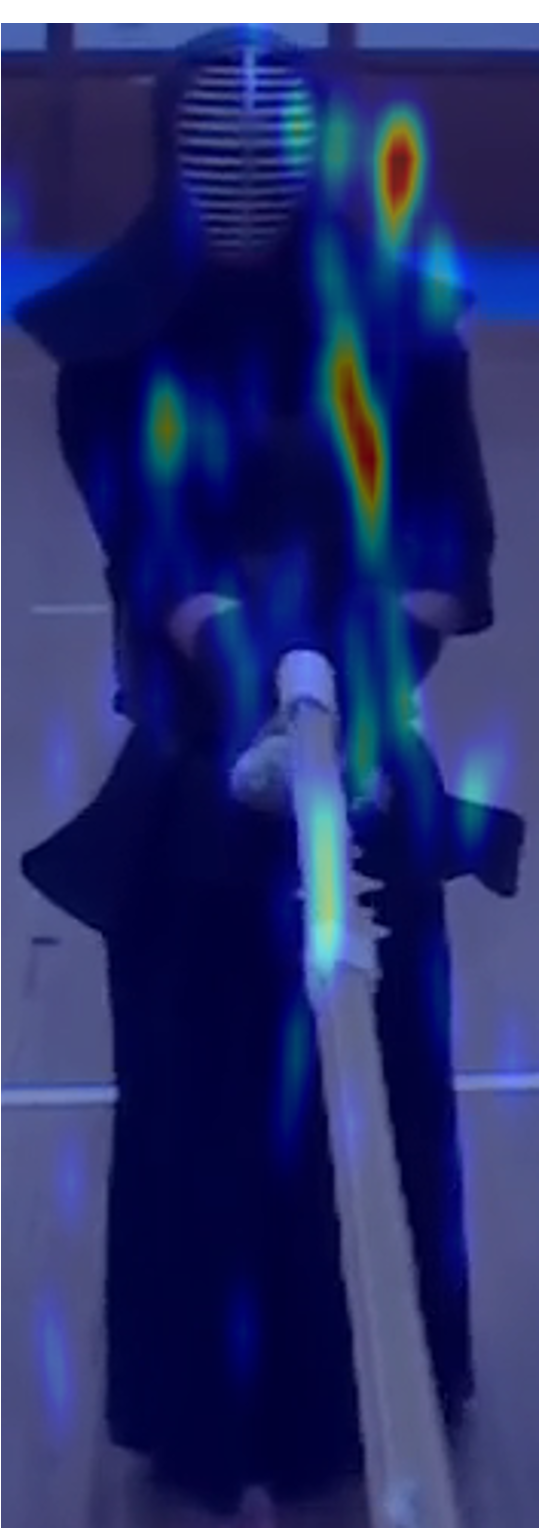
\includegraphics[width=\linewidth]{kcct-kc-08_head1__heatmap2_1.png}
        \par\vspace{2mm}
        (D)
    \end{minipage}

    \vspace{3mm} % 個別の名前と全体のキャプションの間隔
    \caption{四名の実験協力者における視線情報の比較}
    \label{fig:compare_four_experts}
\end{figure}

    図\ref{fig:compare_four_experts}は、3.1節で説明した手法を用いて
    各実験協力者の打突動作における視線データを累積し、
    ヒートマップとして可視化したものである。
    図において、背景画像は対戦相手の代表フレームであり、
    その上に視線の滞留密度を色情報として重畳している。
    カラーマップは暖色系から寒色系のグラデーションを採用しており、
    暖色の領域ほど動作全体を通じて視線が集中した箇所を示し、
    感触の領域ほど視線の集中が少ない箇所を示している。

    \subsection{考察}
    実験の結果、熟練者の視線は対戦相手の身体中心軸、
    とりわけ頭部から喉元に集中しており、
    「遠山の目付」の実践が定量的に裏付けられた。一方で、
    得意技や身長に応じた視線配置の個人差も確認された。
    これは、熟練者が画一的な一点を見ているのではなく、
    「相手の中心を捉え続ける」という基本原則を遵守しつつ、
    自身の身体的特徴や攻撃スタイルに合わせて、
    視線戦略を最適化していることを示唆している。
    
\section{VRシステムの動作検証}
    生成された映像をUnityに取り込み、
    Meta Quest3上にVR空間として構築・転送した。
    図\ref{fig:vr_view}に実際に動作している
    VRゴーグル内の視界イメージを示す。

    \begin{figure}[htbp]
        \centering
        % ここにスライド13枚目などの「VR視界のスクリーンショット」を入れる
        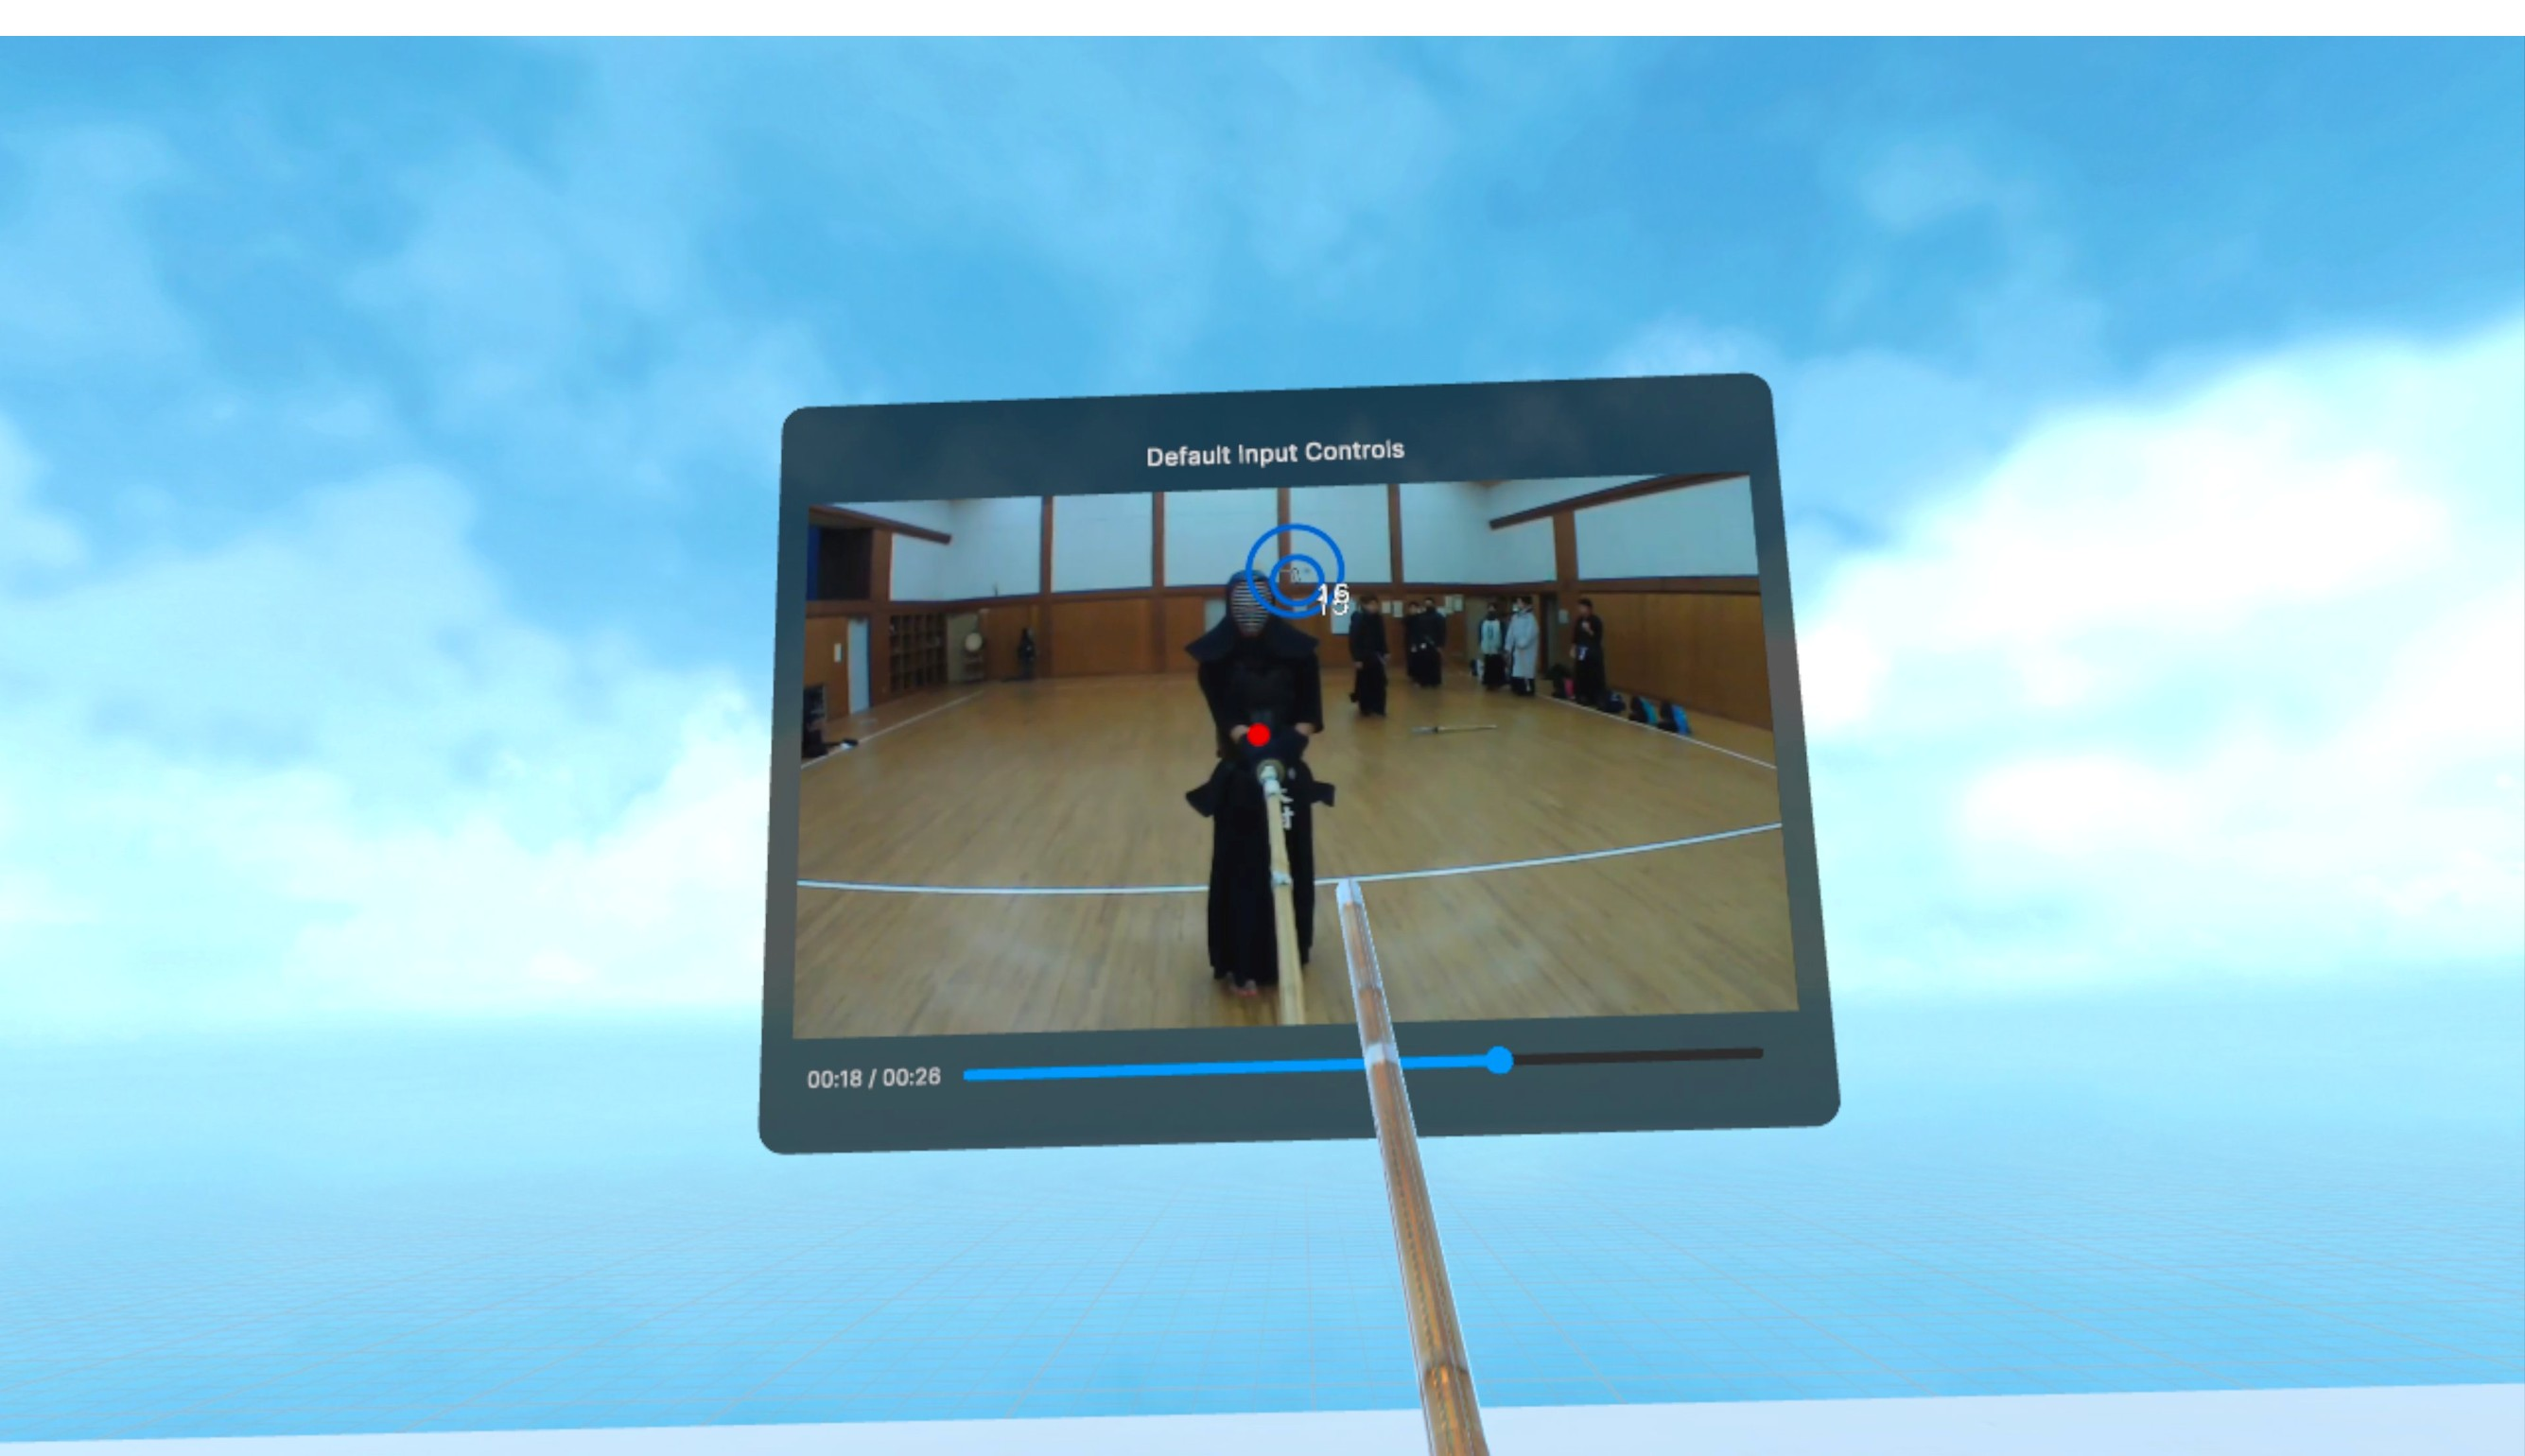
\includegraphics[width=1\columnwidth]{image_20_1.jpg} 
        \caption{Meta Quest3でのVR視界イメージ}
        \label{fig:vr_view}
    \end{figure}

\section{まとめ}
%\subsection{考察}
%実験により、熟練者が「遠山の目付」を基本としつつ、
%得意技に応じて視線戦略を最適化していることが明らかになった。
%本研究は、熟練者の暗黙知である視線技術をデジタル化して可視化するものであり、
%経験や感覚に依存しない新たな技能伝承の手法を確立したといえる。

%実験の結果、熟練者の視線は正中線に集中し、
%「遠山の目付」の実践が定量的に裏付けられた。
%一方で、熟練者が画一的な一点を見つめているのではなく、
%自身の身体的特徴や得意技といった属性に応じて、
%無意識的に情報の取得効率が最大化する位置に視線の
%基準点を調整していることを
%示唆された。
%本システムは、
%言語化困難な熟練者の「暗黙知」をYOLOによる解析で「形式知」へと
%変換した点において、新たな技能伝承モデルとして有用である。

本研究では、YOLO等の画像解析により
剣道熟練者の動的な視線配置を定量化、可視化することができた。
また、VRトレーニングシステムの実施のための環境構築も完了した。
今後の課題として、以下の3点がある。

第一に、熟練者の個人差を考慮した学習モデルの構築である。
確認された視線戦略の多様性を類型化し、
学習者の特性や目標に合わせた最適なモデルを選択できる仕組みが必要である。

第二に、MR技術による自己身体の視認性向上である。
現状のVRでは自身の竹刀が見えないため、リアルタイムの手元映像を表示し、
自分の構えと熟練者の視線を同時に確認できる環境への拡張が求められる。

第三に、データ抽出における時間的同期の精度向上である。
打突時の動作変化を基準とした現状の抽出手法では
微細なズレが生じる懸念があるため、今後はより適切な終了点を模索し、
データの信頼性を高める必要がある。

%第一に、熟練者の個人差を考慮した学習モデルの構築である。
%本実験で確認された視線戦略の多様性を類型化し、
%学習者が自身の特性や目標とするスタイルに合わせて最適なモデルを
%選択できる仕組みが必要である。

%第二に、MR 技術による自己身体の視認性向上である。
%現状の VR 空間では学習者自身の竹刀が見えないため、
%ビデオパススルー機能等を活用して実写の手元映像を合成し、
%自分の構えと熟練者の視線を同時に確認できる環境への拡張が求められる。

%第三に、データ抽出における時間的同期の精度向上である。
%本解析では打突時の激しい動作変化を基準に終了点を定めたが、
%この手法では微細なタイミングのズレが生じ、
%データの信頼性に影響する懸念がある。
%今後は終了点をどこにするかを模索し、
%データに大きな差異が出ないようにする必要がある。


\begin{thebibliography}{99}%参考文献
\bibitem{torigoe} Y. Torigoe, et al.: ``Strike Activity Detection and Recognition Using Inertial Measurement Unit towards Kendo Skill Improvement Support System'', Sensors and Materials, Vol.32, No.3, pp.943-953 (2020).

\bibitem{jeong} K. Jeong, et al.: ``Pressure Sensors for Measuring the Grip Pressure during Kendo Attacks: Assessment of Laterality and Evidence of the Five Phases of Attack'', Sensors, Vol.23, No.3, 1189 (2023).

\bibitem{akiyama} 秋山大輔, 他: ``大学生剣道競技者の面技における視線配置-目付けの教えと基本技稽古の目付けに着目して-'', スポーツパフォーマンス研究, Vol.8, pp.388-397 (2016).

\end{thebibliography}

\end{document}
